%%
%% This is file `example/ch_intro.tex',
%% generated with the docstrip utility.
%%
%% The original source files were:
%%
%% install/buptgraduatethesis.dtx  (with options: `ch-intro')
%%
%% This file is a part of the example of BUPTGraduateThesis.
%%

\chapter{探索使用数据集全局信息指导神经网络Dropout方式}

\section{引言}
神经网络在自然语言处理中取得了显著成果。
然而,考虑到计算复杂性和空间限制,神经网络通常通过mini-batch(批处理)来训练。而mini-batch处理中,由于他不能在一个批次中看到整个全局的情况,模型其实是在隐式地收集全局信息。为了促进学习过程,\citecf{li2017initializing}从训练数据集中提取全局语义特征,并使用新颖的初始化机制将它们作为CNN的初始卷积核。这种方法在情感分析和主题分类任务等方面都获得了显著提高。

与大多数机器学习方法不同,神经网络的优势在于无需进行特征工程就可以提取特征。通常,模型自动学习特征的能力越强,它最终的分类效果就会越好。但是,在训练过程中,神经网络通常倾向于专注于一些具有显著区分性的单词或短语,而忽略其他值得注意的特征。这可能会导致模型对一部分特征过拟合,而对其他一些特征学习的不全面。这种现象在在较小的数据集中尤为明显。为避免此问题,一些学者提出了dropout(丢弃)的想法,其关键思想是在训练过程中从神经网络中随机丢弃单元,并在测试中全部使用学好的单元\cite{hinton2012improving,srivastava2014dropout}。

受上述想法的启发,我提出了一种受全局信息指导的新型丢弃方法(GI-Dropout)。在我们的方法中,我们通过丢弃那些区分性强且易于学习的词,来迫使模型更加关注那些不显著、难学习的特征。

不同于传统的丢弃方法,即以相同的概率随机丢弃神经元,我们将全局信息编码为丢弃率。
具体来说,我们基于单词的重要性丢弃单词,这些单词是通过我们提出的改进的的Naive Bayes(NB)加权技术,并从训练数据中计算得到的。
通过这种丢弃方法,神经网络不仅可以提取显著区分性强的特征,而且还会充分挖掘其他不显著的特征,提高网络的分类性能。

我们在最经典的两个分类基线模型上进行了实验,实验发现集成了我们GI-Dropout方法的模型,可以在几个基准数据集上取得很大提升。且我们的方法很简单,不需借助外部知识库,也很容易和其他深度模型进行结合。


\section{GI-Dropout方法}
我们的动机很容易理解。
由于神经网络旨在捕获语义特征并根据其语义特征对句子进行分类,我们鼓励模型尽可能的学习更多的特征(尤其是那些不那么显著的特征)。我们的方法是,通过计算每个单词对分类的显著性,在神经网络训练的过程中,将显著性高的单词以一定的概率丢弃,从而迫使模型多去学习那些不显著的特征。
有一些特征非常的具有区分性,使得模型可以很容易地学习它们。但是,一个句子可能具有不止一个有助于类别预测的特征。
例如,在``The story is sad and very boring''中,``boring''具有强烈的极性并表示负面情绪。
而由于``boring''的强烈影响,神经网络会``偷懒'',因为他只要看见``boring''就能做正确的判断,这使得神经网络将没有动力去学习同样有助于分类的``sad''特征。
基于这个想法,我们提出了GI-Dropout中,在训练过程中,使得显著性较高的单词有一定的概率被丢弃,从而迫使模型学习其他特征,而在预测时,使用全部特征,从而获得更好的性能。


\subsection{重要性分数}
\label{Importance Score}
首先,我们需要计算每个单词的重要性得分。
从直觉上讲,``unique(独特)''一词在确定影评态度上时比``movie(电影)''重要得多。
Na\"ive Bayes (NB) weighting(朴素贝叶斯加权)是一种确定单词重要性的方法\cite{martineau2009delta,wang2012baselines,li2017initializing}。
类$c$中单词$w$的NB权重$\emph{r}$计算如下:

\begin{equation}\label{tra_nb}
 \emph{r}_{c}^{w} = \frac{(\emph{n}_{c}^{w} + \alpha ) /\left \| \emph{n}_{c} \right \|_{1}} {(\emph{n}_{\tilde{c}}^{w} + \alpha )/\left \| \emph{n}_{\tilde{c}} \right \|_{1}}
\end{equation}
其中 $\emph{n}_{c}^{w}$是单词$w$在类别$c$的频数,
$\emph{n}_{\tilde{c}}^{w}$ 是单词$w$在其他类别中的频数,
$\left \| \emph{n}_{c} \right \|_{1}$是$c$中其他所有单词的频数之和,
$\left \| \emph{n}_{\tilde{c}} \right \|_{1}$是其他类别中所有单词的频数之和,
$\alpha$是用来保证除法有意义的项,在本文中设为了1。 

为了避免将低频单词识别为重要单词,我们提出了一种基于(\ref{tra_nb})的改进的NB加权方法,其中 $\log_{\beta}\emph{n}_{c}^{w}$ 是频率因子,$\beta$ 是一个超参。


\begin{equation}\label{new_nb}
  \emph{r}_{c}^{w} = \frac{(\emph{n}_{c}^{w} + \alpha ) /\left \| \emph{n}_{c} \right \|_{1}} {(\emph{n}_{\tilde{c}}^{w} + \alpha )/\left \| \emph{n}_{\tilde{c}} \right \|_{1}} \times \log_{\beta}\emph{n}_{c}^{w}
\end{equation}


对于电影评论数据集(MR)中的感情正类中,``unique(特别)''和``warm(温暖)''等单词的分数应该大一些,因为它们在感情正项的文章中比在感情负向的文章中更频繁地出现。
至于诸如``the(定冠词)''和``movie(电影)''之类的中性词,它们的分数应该很小,因为他们的出现和类别相关性不大,不具备区分性。
对于单词$w$,我们选择其最高得分作为其重要性得分:
\begin{equation}\label{final_score}
  \emph{r}^{w} = max(\emph{r}_{c_{0}}^{w}, \emph{r}_{c_{1}}^{w}, ..., \emph{r}_{c_{n}}^{w})
\end{equation}

\begin{figure}[!t]figure
\centering
\includegraphics[width=\linewidth]{figure/cr_map.pdf}
\caption{客户评论数据集中最重要的30个词}
\label{fig: keyword}
\end{figure}
在图\ref{fig: keyword}中,我们展示了客户评论数据集(CR)中每个类别的前30个关键字。
我们希望以更高的概率在模型训练过程中丢弃这些关键词,从而鼓励模型更多地关注其他区分性不强的单词(特征)。

\subsection{丢弃率}
\label{dropout rate}
\begin{figure}[!t]
\centering
  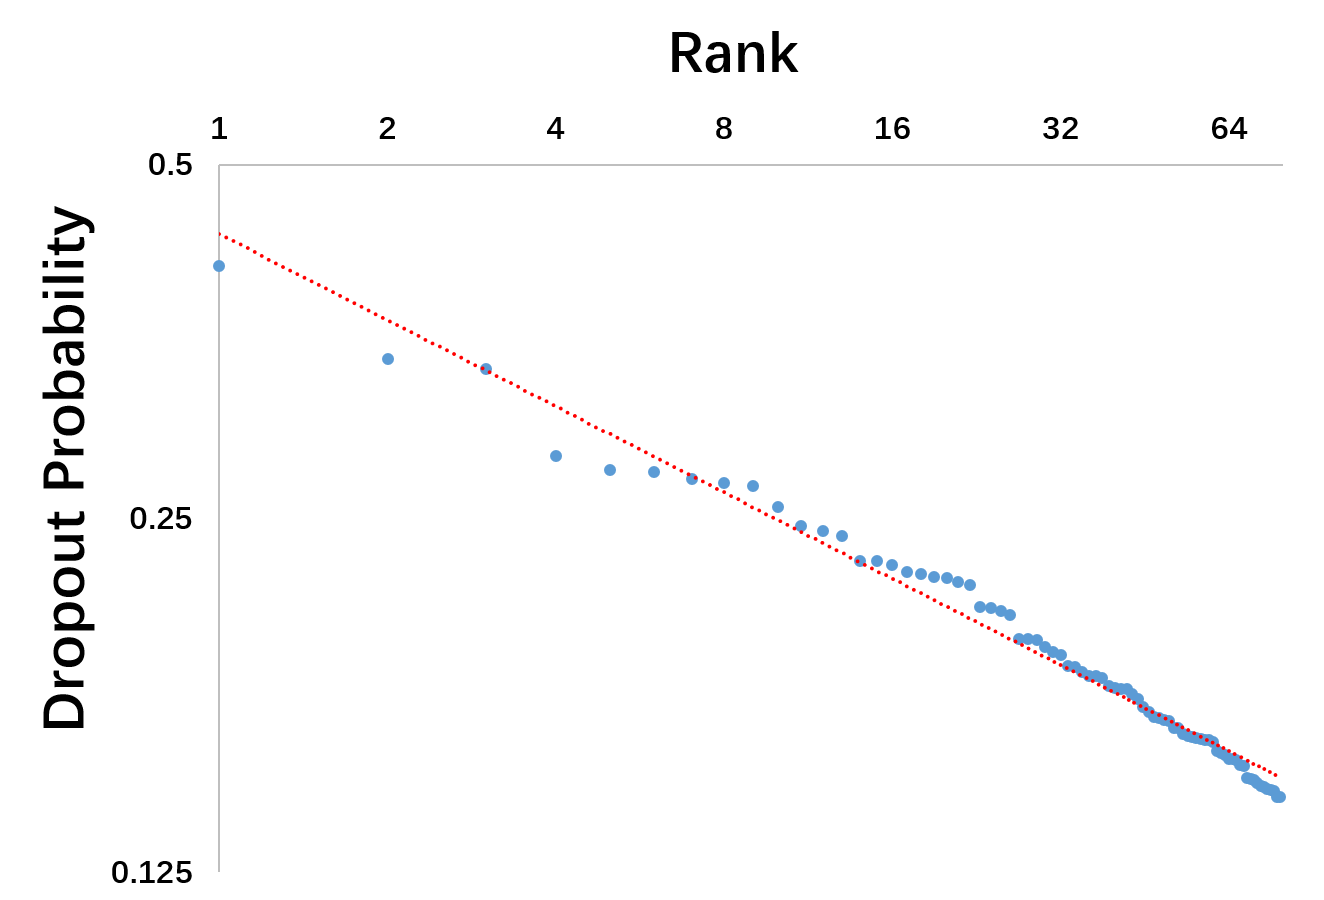
\includegraphics[width=\linewidth]{figure/zipf.png}
  \caption{GI-Dropout probability and rank in SST-1 with $\beta = 0.95$.}
  \label{fig:zipf}
\end{figure}

如\ref{Importance Score}所示,我们使用整个训练数据集计算单词的重要性分数,这是一种简单而有效的表示全局信息的方法。得到分数后,我们将其压缩到$[0, 1)$。单词$w$的丢弃概率如下,其中$r$ 是$w$通过(\ref{new_nb})计算出的。对于一个句子,如果其中一个词的丢弃率为0,则说明该词永远不会被丢弃,即在每一次该句的训练中,这个词永远都会被保留。
\begin{equation}
\label{equation:our fuction}
p(r) = \frac{e^{r} - 1}{e^{r} + 1}
\end{equation}

\ref{new_nb}中的$\beta$是一个关键参数,如图\ref{fig:zipf}所示,在调整$\beta$之后,单词的GI-Dropout概率及它的频数排名遵循Zipf's律。
\citecf{zipf1935psychology}指出,给定一个单词样本,任何单词的频率都与它在频率表中的排名成反比。
用GI-Dropout概率代替频率,我们可以得到Zipf's定律的一个变种。
后续实验将表明,在SST-1中将$\beta$设置为此值并非巧合。

\subsection{GI-Dropout方法}
\begin{figure}[!t]
\centering
  \includegraphics[width=\linewidth]{figure/gi.pdf}
  \caption{GI-Dropout方法. 在这个例子中,单词``boring''的词向量被丢弃因而被设为了0向量,而单词``sad''的向量保留了。}
  \label{fig: model}
\end{figure}

如图\ref{fig: model}中所示,我们在神经网络之前加入了GI-Dropout层。
没有加入我们GI-Dropout的模型可以被视为特殊情况,即其中所有单词都不会在GI-Dropout层中被丢弃,即所有单词的dropout rate均为0。

在本文中,训练数据中的每个单词都有一个分数,可以通过前面介绍的新的NB加权方法得到该分值,并通过\ref{dropout rate}中的函数计算出的丢弃率。
在训练过程中,单词将根据其丢弃率被丢弃。

实现我们GI-Dropout的方法非常简单。
在嵌入层中,通过在嵌入表中查找后,我们得到单词$w_{i}$的嵌入$e_{i}$。之后,我们根据其GI-Dropout的概率将其删除。
对于单词$w_{i}$ ,如果需要删除,我们就将它的向量$e_{i}$设置为零向量。
通过这种方法,神经网络将不会从嵌入为零向量的单词中学习特征。

需要注意的是,与传统的丢弃方法不同,在我们的方法中,每个单词的丢弃率彼此不同,而传统的丢弃方法是根据相同的概率来丢弃所有神经元的。
这些不同的丢弃率,正是整个数据集全局信息的体现,可以指导模型更加关注那些非显著的特征。
 
此外,在传统的丢弃方法中,所有神经元都用于测试,但是它们的权重会按$p$的比例缩小(与训练中的$p$相同)。
在我们的方法中,在评估和测试过程中,所有单词的丢失概率都设置为0,以便模型捕获所有对分类有意义的特征,并且不需要对这些值进行缩放。


\section{实验}
\subsection{数据集}
跟随\citep{kim2014convolutional}的工作,我们在7个常用的文本分类数据集上评估了我们提出的方法,包括情感分类、主题分类等文本分类数据集。

\begin{table}[!t]
% \renewcommand{\arraystretch}{1.3}
\centering
\begin{tabular}{c c c c c c}
\hline
\bfseries 数据集 & 类别数 & 句子长度 & 数据集大小 & 词表大小  & 测试集\\
\hline
MR & 2 & 20 & 10662 & 18765 &  交叉验证\\
SST-1 & 5 & 18 & 11855 & 17836  & 2210\\
SST-2 & 2 & 19 & 9613 & 16185  & 1821\\
Subj & 2 & 23 & 10000 & 21323  & 交叉验证\\
TREC & 6 & 10 & 5952 & 9592  & 500\\
CR & 2 & 19 & 3775 & 5340  & 交叉验证\\
MPQA & 2 & 3 & 10606 & 6246 & 交叉验证\\
\hline
\end{tabular}
\caption{\ 数据集介绍整体情况概述,交叉验证指该数据集没有明确区分训练集、测试集,因此我们用交叉验证的方式进行结果检验。}
\label{table: dataset summary}
\end{table}

\textbf{MR}: 电影评论数据集\footnote{https://www.cs.cornell.edu/people/pabo/movie-review-data/}.

\textbf{SST-1}: 斯坦福发布的情感分类数据集(五分类\citep{socher2013recursive}\footnote{http://nlp.stanford.edu/sentiment/}。 数据集包括短语级别、句子级别的分类实例. 为了和\citep{kim2014convolutional}的结果保持一致,  我们的训练集包含短语级别和句子级别的所有句子,但是只在句子级别的实例中进行测试。

\textbf{SST-2}: 和SST-1数据集一样,不同的是,将5分类问题变成了更简单的二分类问题。

\textbf{Subj}: 主观及客观分类数据集 \citep{pang2005seeing}。

\textbf{TREC}: 问题分类数据集 \citep{li2002learning} \footnote{http://cogcomp.cs.illinois.edu/Data/QA/QC/}.

\textbf{CR}: 用户购买产品评论数据集 \citep{hu2004mining} \footnote{http://www.cs.uic.edu/∼liub/FBS/sentiment-analysis.html}.

\textbf{MPQA}: 观点极性检测数据集 \citep{wiebe2005annotating}.

数据集的概述请见表\ref{table: dataset summary}。
\subsection{GI-Dropout引入CNN}
\begin{figure}[!t]
\centering
  \includegraphics[height=0.5\textheight]{figure/CNN_vertical_new_with_GI.pdf}
  \caption{GI-Dropout引入CNN模型}
  \label{fig: cnn}
\end{figure}

\begin{table}[!t]
% \renewcommand{\arraystretch}{1.3}
\centering
\begin{tabular}{c c}
\hline
\bfseries Parameters & \bfseries Values\\
\hline
词向量 & GoogleNews-negative300 \\
是否微调词向量 & 是\\
卷积方式 & 1-d \\
卷积核大小 & [3, 4, 5] \\
卷积核数量 & 300 \\
激活函数 & ReLU \\
池化方法 & 最大池化 \\
Dropout值 & 0.5 \\
\hline
\end{tabular}
\caption{CNN模型参数设定.}
\label{table: baseline hyperparameters}
\end{table}

CNN模型使用卷积核捕获n-gram的语义特征。
随后,使用最大池化的方法以强制神经网络关注卷机核捕获的最有用的局部特征\cite{collobert2011natural}。
\citecf{kim2014convolutional}提出了一个简单的CNN模型用于文本分类,包括嵌入层,一个卷积和池化层以及一个全连接层。\citecf{kim2014convolutional}提供了四个模型变体,我们选择其中的CNN-non-static模型作为基线模型。
CNN的超参数在表\ref{table: baseline hyperparameters}中进行了描述,其中GoogleNews-negative300是公开的在Google News上使用word2vec\cite{mikolov2013distributed}训练的300维词向量。
而在此基础之上,集成了我们提出的GI-Dropout的模型架构如图\ref{fig: cnn}所示。
该模型相比于baseline除了我们加到第一层的GI-Dropout层,其他都完全一样,希望通过这种方法来测试GI-Dropout的效果。

\subsection{Self-attentive RNN Model}
\begin{figure}[!t]
\centering
  \includegraphics[height=0.8\textheight]{figure/self+attention+new.pdf}
  \caption{Self-attentive RNN architectures.}
  \label{fig: rnn}
\end{figure}

长短期记忆网络(LSTM)是一种特定的递归神经网络(RNN)架构,擅长对时间序列进行建模,并且可以捕获长期依赖性\citep{sak2014long}。
注意力机制最早在\citep{bahdanau2014neural}中提出,现已成为序列建模中应用非常广泛的组成部分。
\cite{lin2017structured}提出的Self-attentive RNN由双向LSTM(bi-LSTM)和自注意力机制(self-attention)组成。
自注意力机制用于替换biLSTM之后的最大池化或平均池化,从而可以对句子各部分的语义特征进行整合,更好的对该句进行建模。
假设我们有一个$n$个单词的句子,并且使每个LSTM单元的隐藏大小为$u$。
在bi-LSTM层之后,我们可以获得输出$H$,其大小为$n$*$2u$。
自注意力机制将整个LSTM隐藏状态$H$作为输入,并输出权重向量$a$,
\begin{equation}
\emph{a} = softmax(w_{s2}\tanh(W_{s1}H^T))
\end{equation}
其中$W_{s1}$是权重矩阵,形状为$d_{a}$*$2u$,$W_{s2}$是大小为$d_{a}$的超参数向量。

为了提取句子中$r$的不同方面,\cite{lin2017structured}提出多重注意力,即将$w_{s2}$扩展成$r$*$d_{a}$矩阵,并将其记为$W_{s2}$。
最后,权重向量$a$成为权重矩阵$A$。

\begin{equation}
\emph{A} = softmax(W_{s2}\tanh(W_{s1}H^T))
\end{equation}

则句子的向量为:
\begin{equation}
\emph{M} = \emph{A}\emph{H}
\end{equation}
然后,该论文使用具有带ReLU激活函数的两层MLP(全连接层)来预测句子的标签。此外,引入了惩罚项以鼓励不同关注力权重对句子关注的多样性。

\begin{table}[!t]
% \renewcommand{\arraystretch}{1.3}
\centering
\begin{tabular}{c c}
\hline
\bfseries 参数 & \bfseries 值\\
\hline
词向量 & Glove-300 \\
是否微调词向量 & 是\\
biLSTM隐层大小 & 300 \\
$d_{a}$ & 350 \\
$r$ & 4 \\
全连接层激活函数 & ReLU \\
全连接层Dropout值 & 0.5 \\
\hline
\end{tabular}
\caption{Self-attentive RNN参数设置.}
\label{table: self-attention baseline hyperparameters}
\end{table}

由于\citecf{lin2017structured}不提供源代码,因此我们自己复现了模型,并将GI-Dropout集成到模型中,如图\ref{fig: rnn}所示。
我们执行grid search(参数网格搜索)以获取基线模型的最佳超参数,且该超参数可以在大多数数据集中取得最佳效果。
该模型使用bi-LSTM,每个方向上的隐藏状态维度为$300$。
在自注意力机制部分,$d_a$为$350$,惩罚项的系数为$1$。
考虑到数据集的大小和文本的长度,我们将$r$设置为$4$。
我们还使用隐藏单元为2000,带ReLU激活函数的两层MLP(全连接层)作为输出层。
在训练期间,MLP上的dropout值为$0.5$。
表\ref{table: self-attention baseline hyperparameters}中描述了这些超参数。其中Glove-300是预训练好的300维的公开词向量\citep{pennington2014glove}


\subsection{实验设置}
我们将GI-Dropout方法应用于上述提到的两个基线模型。
为了公平地比较,集成了GI-Dropout方法的模型和基线模型使用相同的超参数设置。数据集方面,无论是基线模型还是我们提出的模型,都严格按照训练集训练,验证集选取最优模型,测试集测试进行训练测试。对于没有测试集的数据集,我们将其拆分并以固定的随机种子进行交叉验证。我们使用早停方式,并将早停值设为10。

\subsection{实验结果}

\begin{table*}[t]
\begin{small}
% \begin{singlespace}
\tabcolsep=0.11cm

% \renewcommand{\arraystretch}{1.3}
\centering
\begin{tabular}{c |ccccccc}
\hline
\bfseries Model             & MR   & SST-1 & SST-2 & Subj & TREC &  CR  & MPQA\\
\hline
CNN-non-static & 81.5 & 48.0  & 87.2  & 93.4 & 93.6 & 84.3 & 89.5\\
\hline
CNN-reproduce       & 81.4 & 47.8  & 87.5  & 93.0 & 92.4 & 84.3 & 89.6\\
CNN-Dropout-same (p)       &  81.5(0.1) & 48.5(0.1)  & 87.6(0.1)  & 93.5(0.2) & 92.9(0.1)& 84.5(0.5) & 87.4(0.1)\\

CNN-GI-Dropout ($\beta$) & \textbf{81.9}(0.87) & \textbf{49.0}(0.95)  & \textbf{88.1}(0.98)  & \textbf{93.4}(0.91) & \textbf{93.2}(0.83) & \textbf{85.1}(0.87) & \textbf{89.8}(0.98)\\

\hline
\hline
RNN-baseline & 82.1 & 49.7  & 89.7  & 93.6 & 92.6 & 84.1 & 89.6\\
RNN-Dropout-same (p) & 82.2(0.2) & 51.9(0.1)  & 90.1(0.1)  & 93.9(0.1) & 93.4(0.2) & 84.2(0.1) & \textbf{89.7}(0.1)\\
RNN-GI-Dropout ($\beta$) & \textbf{82.5}(0.87) & \textbf{54.1}(0.95)  & \textbf{90.4}(0.95)  & \textbf{94.2}(0.98) & \textbf{94.8}(0.95) & \textbf{84.7}(0.91) & \textbf{89.7}(0.98)\\

\hline
\hline
MVCNN & - & 49.6 & \underline{89.4} & 93.9 & - & - & -\\ 
MGNC-CNN & - & 48.7 & 88.3 & \underline{94.1} & 95.5 & - & -\\ 
CNN-Rule & 81.7 & - & 89.3 & - & - & 85.3 & -\\ 
Semantic-CNN & 82.1 & 50.8 & 89.0 & 93.7 & 94.4 & \underline{86.0} & \underline{89.3}\\ 
combine-skip & 76.5 & - & - & 93.6 & 92.2 & 80.1 & 87.1\\ 
DSCNN & \underline{82.2} & 50.6 & 88.7 & 93.9 & \underline{95.6} & - & -\\ 
Paragraph Vector & 74.8 & 48.7 & 87.8 & 90.5 & 91.8 & 78.1 & 74.2\\ 
NBSVM & 79.4 & - & - & 93.2 & - & 81.8 & 86.3\\ 
Tree LSTM & - & \underline{51.0} & 88.0 & - & - & - & -\\ 
\hline
\end{tabular}

\caption{GI-Dropout的效果.
Dropout-same表示以同样的概率丢弃每个单词,括号中的值代表丢弃概率的大小。
我们同样提供了其他经典方法在这些数据集上的结果: MVCNN \cite{yin2015multichannel}, MGNC-CNN \cite{zhang2016mgnc}, CNN-Rule \cite{hu2016harnessing}, Semantic-CNN \cite{li2017initializing}, combine-skip \cite{kiros2015skip}, combine-skip \cite{kiros2015skip}, DSCNN \cite{zhang2016dependency}, Paragraph Vector \cite{le2014distributed}, NBSVM \cite{wang2012baselines} 以及 Tree LSTM \cite{tai2015improved}.
}
\label{table: result}
\qquad
% \end{singlespace}
\end{small}
\end{table*}

表\ref{table: result}中列出了7个数据集上的实验结果。
实验表明,引入了GI-Dropout的模型明显优于CNN和self-attentive RNN基线模型。

为了测试全局信息是否做出了重要贡献,我们进行了另一个实验,即在GI-Dropout层根据相同的概率删除所有单词。我们使用了grid search(网格搜索)方法用于寻找最佳的删除概率值,并将最佳结果列在``Dropout-same-prob''行中。

简单的CNN模型提供了非常强的基线结果。
在表格中,第一行是论文\cite{kim2014convolutional}中CNN-non-static的原始结果。
``CNN-baseline''是我们自己复现该模型的实验结果。

表\ref{table: result}显示,通过简单地根据相同的概率删除所有单词,除MPQA之外,该模型相对于所有数据集的CNN基线都有轻微的改进。同样,与大多数数据集的self-attentive RNN基线模型相比,它也可以带来一些收益。

而通过集成我们的GI-Dropout机制,我们进一步提高了CNN和RNN模型的性能。与Dropout-same相比,在全局信息指导下的Dropout在所有数据集上的结果都得到了改善。
通过比较GI-Dropout和Drop-same,我们确信GI-Dropout受益于全局信息,该信息提供了明确的语义信息来指导训练过程。
即使与具有复杂结构的其他模型相比,GI-Dropout模型也可以在大多数数据集上达到最佳性能,尤其是在SST-1和SST-2数据集中。

\section{结果深入分析}

\subsection{GI-dropout 帮助模型学习不显著特征}
\begin{table}[!t]
% \renewcommand{\arraystretch}{1.3}
\centering
\begin{tabular}{c | c c}
\hline
\bfseries Top-k &  CNN baseline &  GI-Dropout in CNN\\
\hline
0 & 87.5 & 88.1  \\
50 & 87.1 & 87.9  \\
100 & 86.7 & 87.9  \\
200 & 86.1 & 87.5  \\
500 & 84.7 & 86.6  \\
1000 & 81.7 & 84.0 \\

\hline
\hline
\end{tabular}
\caption{在SST-2数据集中,当我们移去top-k关键词后的准确率下降趋势。}
\label{table: decline-SST-2}
\end{table}
为了测试该方法是否确实有助于模型学习不明显的特征,我们进行了如下实验,即从“ SST-2”的测试用例中删除了前k个显著词(具有最高重要分数的词),观察他的效果。
结果显示在表\ref{table: decline-SST-2}中。
我们可以观察到CNN baseline模型对显著特征更为敏感,而相反,即使删除了前1000个显著词,引入了GI-Dropout的模型仍然可以取得相对较好的结果。
因此,GI-Dropout可以帮助模型更加关注那些不显著的特征。


\subsection{GI-dropout 帮助模型减少对显著特征的过拟合}
我们都知道,频繁出现的一些单词很容易使模型专注于某一些特征,并且在全连接层只激活分数较高的部分单元。我们从测试用例中挑选了部分baseline模型做错,而GI-Dropout模型做对的用例,并进行进一步分析。示例中,\textbf{加粗}的单词代表那些有着高分的显著词, 例如在\textbf{positive}中出现了159次而只在\textbf{negative}出现了5次的``pretentious". \underline{下划线}的单词代表了那些非显著的,但是也对分类有贡献的单词。 

\textbf{(1)}  \textit{provide -lrb- s -rrb- nail-biting suspense and credible characters \underline{without} relying on technology-of-the-moment technique or \textbf{pretentious} dialogue.}

\textbf{(2)}  \textit{the screenplay \underline{sabotages} the movie's \textbf{strengths} at almost every juncture.} 

\textbf{(3)}  \textit{this is \underline{cool}, \underline{slick} stuff, ready to \underline{quench} the thirst of an audience that \textbf{misses} the summer blockbusters.} 

baseline模型倾向于关注那些非常显著且起决定作用的特征。如例1的\textbf{``pretentious"} (消极性), 例2的\textbf{``strengths"} (积极性)和例3的\textbf{``miss"} (消极性)。由于对这些非常显著特征的过拟合,且忽视了例1的\textbf{``without"}, 例2的\textbf{``sabotages"}, \textbf{``cool"}, \textbf{``slick"} 和例3的 \textbf{``quench"},baseline模型没有好好利用整句话中的所有信息,导致分类错误。
当引入了GI-dropout方法后,模型不但能学会到\textbf{``strengths"}这种显著特征,也会学习到\textbf{``sabotages"}这种不显著特征,使得该模型能够就行正确的分类。

\subsection{Zipf's Law}

% \begin{figure}[!t]
% \centering
%   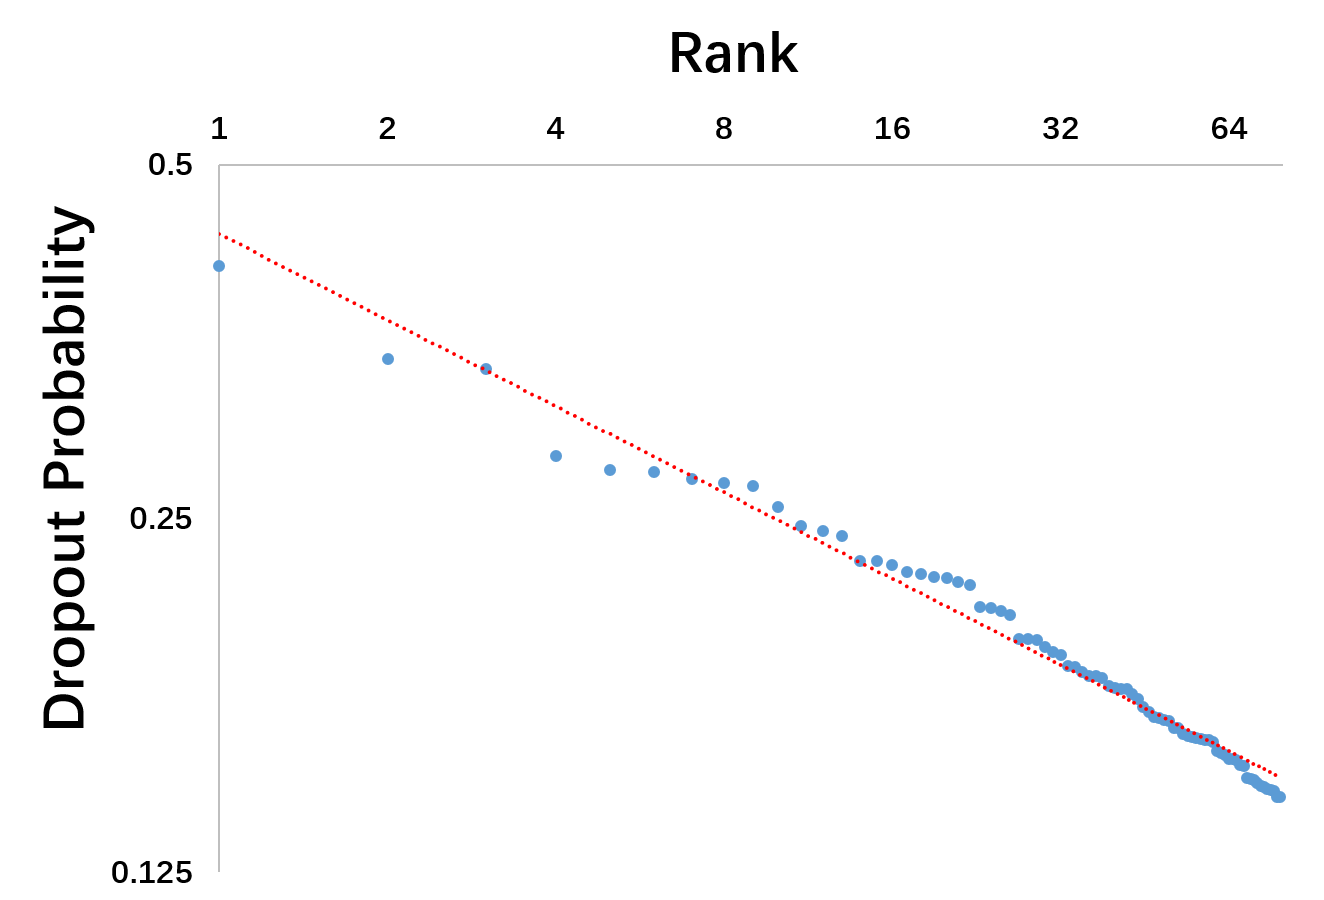
\includegraphics[width=\linewidth]{figure/zipf.png}
%   \caption{当$\beta = 0.95$时,数据集SST-1中,GI-Dropout中单词概率和频率排名的关系。}
%   \label{fig:zipf}
% \end{figure}

\begin{table}[!t]
% \renewcommand{\arraystretch}{1.3}
\centering
\begin{tabular}{c | c c}
\hline
\bfseries $\beta$ & CNN &  RNN\\
\hline
0.98 ($10^{-0.01}$) & 48.8 & 51.9 \\
0.95 ($10^{-0.02}$) & \textbf{49.0} & \textbf{54.1} \\
0.91 ($10^{-0.04}$) & 48.0 & 51.8 \\
0.87 ($10^{-0.06}$) & 48.1 & 52.4 \\
0.83 ($10^{-0.08}$) & 47.4 & 51.4 \\

\hline
\hline
\end{tabular}
\caption{$\beta$ and accuracy in SST-1. }
\label{table: SST-1}
\end{table}

此外,我们对于超参$\beta$的取值进行了分析。如图\ref{fig:zipf}所示,当$\beta$的值为0.95时,在数据集SST-1中,每个单词的dropout概率和他的排名近似符合Zipf's Law。事实上,在每一个数据集中,都存在一个准确的$\beta$,使得单词的dropout的概率和其在数据集中词频的排名近似符合Zipf's Law,且这个$\beta$就是让模型达到最好效果的$\beta$。我们认为,这是因为Zipf's Law反映了词重要性和词频的客观规律,根据这一定律设置$\beta$值,会更好的体现数据集的特性。为此,我们做了进一步实验,表\ref{table: SST-1}证明了我们的猜想,无论是CNN还是RNN,都是$\beta$值为0.95的时候,GI-Dropout方法取得了最好的效果。


% \begin{enumerate}
% \item 第二章介绍……
% \item ……
% \end{enumerate}

% \chapterbib

